\chapter{Aplicaciones entre Espacios Topológicos}

\begin{definicion}
    Dados $(X, \cc{T})$, $(Y, \cc{T}')$ dos e.t., diremos que $f : (X, \cc{T}) \to (Y, \cc{T}')$ (que notaremos como $f:X \to Y$ cuando estén claros los e.t.) es \textbf{continua} en un punto $x_0\in X$ si $\forall N'\in \cc{N}_{f(x_0)}'$\ \ $\exists N \in \cc{N}_{x_0}$ con $f(N)\subset N'$. 

    \begin{center}
        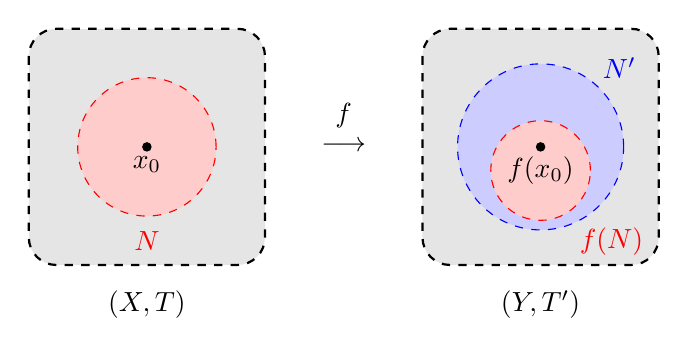
\begin{tikzpicture}
            \def\incolor{gray!20}

            \filldraw[rounded corners=10pt, dashed, thick, fill=\incolor] (0,0) rectangle (3,-3);

            \node at (1.5, -3.5) {$(X, \cc{T})$};
            \node at (4, -1.1) {$f$};
            \node at (4, -1.5) {$\longrightarrow$};

            \filldraw[rounded corners=10pt, dashed, thick, fill=\incolor] (5,0) rectangle (8,-3);

            \node at (6.5, -3.5) {$(Y, \cc{T}')$};

            \filldraw[dashed, draw=red, fill=red!20] (1.5, -1.5) circle (25pt);

            \node at (1.5, -2.7) {\textcolor{red}{$N$}};

            \filldraw[dashed, draw=blue, fill=blue!20] (6.5, -1.5) circle (30pt);

            \filldraw[dashed, draw=red, fill=red!20] (6.5, -1.8) circle (18pt);

            \node at (7.4, -2.7) {\textcolor{red}{$f(N)$}};

            \node at (7.5, -0.5) {\textcolor{blue}{$N'$}};

            \filldraw (1.5, -1.5) circle (1.5pt)  node[below] {$x_0$};

            \filldraw (6.5, -1.5) circle (1.5pt)  node[below] {$f(x_0)$};

            
        \end{tikzpicture}
    \end{center}

    Equivalentemente, $\forall N'\in \cc{N}_{f(x)}'$  $f^{-1}(N')\in \cc{N}_{x_0}$. Es decir, la imagen inversa por f de todo entorno de $f(x)$ en el espacio topológico $\cc{T}'$ es entorno de $x$ en el espacio topológico $\cc{T}$.
    \endsquare
\end{definicion}

\begin{observacion}
    La definición se puede reformular usando abiertos, abiertos básicos o entornos básicos. La demostración queda planteada como ejercicio para el lector. %TODO
    \endsquare
\end{observacion}

\begin{definicion}
    Dados $(X, \cc{T})$, $(Y, \cc{T}')$ dos e.t., $\emptyset \neq A\subset X$. Diremos que $f:X\to Y$ es \textbf{continua en $A$} si es continua en $x$\ \ $\forall x \in A$. Diremos que $f$ es \textbf{continua} si es continua en $X$.
    \endsquare
\end{definicion}

\begin{prop}
    Dados $(X, \cc{T})$, $(Y, \cc{T}')$ dos e.t., $f: X \to Y$. Entonces son equivalentes:
    \begin{enumerate}
        \item[(i)] $f$ es continua.
        \item[(ii)] $f^{-1}(U')\in \cc{T}$\ \ $\forall U' \in \cc{T}$ ($f$ trae abiertos en abiertos).
        \item[(iii)] $f^{-1}(B')\in \cc{T}$\ \ $\forall B'\in \cc{B}'$, donde $\cc{B}'$ es base de $\cc{T}'$.
        \item[(iv)] $f^{-1}(C')\in \cc{C}_{\cc{T}}$\ \ $\forall C' \in \cc{C}_{\cc{T}'}$ ($f$ trae cerrados en cerrados).
        \item[(v)] $f(\overline{A})\subset \overline{f(A)}$\ \ $\forall A \subset X$.
    \end{enumerate}

    \begin{proof}\
        \begin{enumerate}
            \item[(i)$\Rightarrow$(ii)] Supongamos que $f$ es continua. Tomamos $U' \in \cc{T}'$ y tendremos que verificar que $f^{-1}(U')\in \cc{T}$. Sea $x \in f^{-1}(U')$, entonces tendré que ver que $f^{-1}(U')\in \cc{N}_x$. Sabemos que $f(x)\in U' \subset \cc{N}_{f(x)}$. Como $f$ es continua, entonces $\exists U\in \cc{T} $, $x\in U$, $f(U)\subset U' \Rightarrow x \in U \subset f^{-1}(U')$. Como $U\in \cc{T}$, tenemos que $f^{-1}(U')\in \cc{N}_x$. Como esto sucede para un $x$ arbitrario tendremos que se verifica.
            \item[(ii)$\Rightarrow$(iii)] Esta implicación es trivial ya que todo abierto básico es en particular abierto en la topología.
            \item[(iii)$\Rightarrow$(iv)] Sea $C' \in \cc{C}_{\cc{T}'}$, $C'\subset Y$. Tendré que ver que $f^{-1}(C')\in \cc{C}_{\cc{T}}$, lo cual es equivalente a ver que $X \setminus f^{-1}(C')\in \cc{T}$. Sabemos que $X\setminus f^{-1}(C') = f^{-1}(Y\setminus C')$ y $Y\setminus C'\in \cc{T}$. Como $\cc{B}'$ es base de $\cc{T}'$, tenemos que $Y\setminus C'=\bigcup\limits_{i\in I} B_i'$ con $B_i'\in \cc{B}'$\ \ $\forall i \in I$. Entonces tenemos que $f^{-1}(Y\setminus C') = f^{-1}\left(\bigcup\limits_{i\in I}B_i'\right) = \bigcup\limits_{i\in I}f^{-1}(B_i')\in \cc{T}$ por ser unión de abiertos.
            \item[(iv)$\Rightarrow$(v)] Sea $\emptyset \neq A \subset X$, como $\overline{f(A)}\in \cc{C}_{\cc{T}'}$, por (iv) tenemos que $f^{-1}(\overline{f(A)})\in \cc{C}_{\cc{T}}$. Además, $A \subset f^{-1}(f(A))\subset f^{-1}(\overline{f(A)})\in \cc{C}_{\cc{T}}$. Entonces $\overline{A}\subset f^{-1}(\overline{f(A)})$. Al aplicar $f$ tenemos que $f(\overline{A})\subset f(f^{-1}(\overline{f(A)}))=\overline{f(A)}$.
            \item[(v)$\Rightarrow$(iv)] Sea $C' \in \cc{C}_{\cc{T}'}$ y tendremos que ver que $f^{-1}(C')\in \cc{C}_{\cc{T}}$. Para ello veré que coincide con su adherencia, es decir, que $\overline{f^{-1}(C')} = f^{-1}(C')$. Como la inclusión $\overline{f^{-1}(C')} \supset f^{-1}(C')$ es clara tendré que ver solo la otra incusión. Sea $A=f^{-1}(C')$, por (v) tenemos que $f(\overline{f^{-1}(C')})\subset \overline{f(f^{-1}(C'))} \subset \overline{C'}=C'$. Aplicando $f^{-1}$ tenemos que $f^{-1}(f(\overline{f^{-1}(C')}))\subset f^{-1}(C')$ y como $f^{-1}(f(\overline{f^{-1}(C')})) = \overline{f^{-1}(C')}$ tenemos lo buscado.
            \item[(iv)$\Rightarrow$(i)] Sea $x\in X$ arbitrario. Tendré que ver que $f$ es continua en $x$. Sea $U'\in \cc{T}'$ con $f(x)\in U'$. Tendré que ver que existe un $U\in \cc{T}$ con $x\in U$ y $f(U)\subset U'$. Tomo $Y\setminus(U')\in \cc{C}_{\cc{T}'}$ y por (iv) tenemos que $f^{-1}(Y\setminus U')\in \cc{C}_{\cc{T}}$ y $f^{-1}(Y\setminus U') = X \setminus f^{-1}(U')$ por lo que $x\in f^{-1}(U')\in \cc{T}$. Como $f(f^{-1}(U'))\subset U'$ puedo denotar $U = f^{-1}(U')$ y tenemos de nuevo lo buscado. 
        \end{enumerate}
    \end{proof}
\end{prop}

\begin{observacion}
    Si $f: (X, \cc{T}) \to (Y, \cc{T}')$ es una aplicación continua, entonces 
    \begin{gather*}
        f^{-1}((a,b)), f^{-1}((-\infty, b)), f^{-1}((a, +\infty))\in \cc{T}
    \end{gather*}
    y además 
    \begin{gather*}
        f^{-1}([a,b]), f^{-1}((-\infty, b]), f^{-1}([a, +\infty))\in \cc{C}_{\cc{T}}
    \end{gather*}
    La utilidad de esta observación es poder ver si un conjunto es abierto viendo si existe una aplicación continua que lleve un abierto de la topología en dicho conjunto. Análogamente se puede usar para cerrados.
    \endsquare
\end{observacion}

\begin{ejemplo}\
    \begin{itemize}
        \item $f:(X, d) \to (Y, d')$ continua entre espacios métricos 
        \begin{align*}
            \sii &\forall \veps >0\ \ \exists \delta >0 \text{ tal que si } d(x, x_0)<\delta \text{ entonces } d'(f(x), f(x_0))<\veps \sii\\
            \sii &\forall \veps >0 \ \ \exists \delta >0 \text{ tal que } f(B(x_0, \delta))\subset B'(f(x_0), \veps).
        \end{align*}
    \end{itemize}
\end{ejemplo}

\begin{observacion}\
    \begin{itemize}
        \item Cuanto más abiertos hay en $\cc{T}$ y menos en $\cc{T}'$ más fácil es que $f$ sea continua. Por ejemplo, las aplicaciones  
        \begin{align*}
            f:&(X, \cc{T})\to (Y, \cc{T}_t)\\
            f:&(X, \cc{T}_{disc})\to (Y, \cc{T}')
        \end{align*}
        son continuas.

        \item Si $f:(X, \cc{T})\to (Y, \cc{T}')$ es constante, $f(x)=y_0\in Y$\ \ $\forall x \in X$, Sea $U'\in \cc{T}$, entonces
        \begin{gather*}
            f^{-1}=\left\{
            \begin{array}{ccc}
                X & \text{ si }& y_0\in U'\\
                \emptyset & \text{ si } & y_0\notin U
            \end{array}
            \right.
        \end{gather*}

        \item $Id_X : (X, \cc{T}) \to (X, \cc{T}')$ es continua $\sii \cc{T}' \leq \cc{T}$. Por ejemplo, $Id_{\bb{R}}:(\bb{R}, \cc{T}_u)\to (\bb{R}, \cc{T}_S)$ no es continua pero $Id_{\bb{R}}:(\bb{R}, \cc{T}_S) \to (\bb{R}, \cc{T}_u)$ sí lo es.
        \item Si $f:(X, \cc{T})\to (Y, \cc{T}')$ y $g:(Y, \cc{T}')\to (Z, \cc{T}'')$ son aplicaciones continuas, entonces $g\circ f : (X, \cc{T})\to (Z, \cc{T}'')$ es continua.
        \begin{proof}
            Sea $U''\in \cc{T}''$, $(g\circ f)^{-1}(U'') = f^{-1}(g^{-1}(U''))\in \cc{T}$.
        \end{proof}
        \item $f:(X, \cc{T})\to (Y,\cc{T}')$ continua y $\emptyset\neq a  \subset X$, entonces
        \begin{align*}
            f_{|A}:(A, \cc{T}_A) &\to (Y, \cc{T}') \text{ es continua}\\
            x & \mapsto f(x)
        \end{align*}
        \begin{proof}
            Sea $U'\in \cc{T}'$, $(f_{|A})^{-1}(U') = \{x \in A : f(x)\in U\} = f^{-1}(U') \cap A\in \cc{T}_A$ ya que $f^{-1}(U')\in \cc{T}$.
        \end{proof}
        \item Si $f:(X, \cc{T})\to (Y, \cc{T}')$ continua, $\emptyset \neq A' \subset Y$ con $f(X)\subset A'$, entonces 
        \begin{align*}
            f^{A'}:(X, \cc{T}) &\to (A', \cc{T}_{A'}') \text{ es continua}\\
            x &\mapsto f(x)
        \end{align*}
        \begin{proof}
            Sea $O'\in \cc{T}_{A'}'$, entonces $\exists U'\in \cc{T}'$ con $O'=U'\cap A \Rightarrow (f^{A'})^{-1}(O') = (f^{A'})^{-1}(U'\cap A') = f^{-1}(U')\in \cc{T}$ ya que $f$ es continua y $U'$ es abierto en $\cc{T}'$.
        \end{proof}
    \end{itemize}
\end{observacion}

\begin{lema} (de pegado) Sean $(X, \cc{T})$, $(Y, \cc{T}')$ dos e.t. y sea $\{A_i\}_{i\in I}\subset X$ una familia de subconjuntos no vacío de $X$ y $\{f_i:A_i \to Y\}_{i\in I}$ una familia de aplicaciones tales que 
    \begin{enumerate}
        \item[(i)] $\bigcup\limits_{i\in I} A_i =X$.
        \item[(ii)] $f_i=f_j$ en $A_i\cap A_j$\ \ $\forall i,j\in I$ con $A_i\cap A_j \neq \emptyset$. 
        \item[(iii)] $f_i:(A_i, \cc{T}_{A_i})\to (Y, \cc{T}')$ es continua $\forall i \in I$. 
        \item[(iv)] O bien $A_i\in \cc{T}$\ \ $\forall i \in I$ o bien $A_i \in \cc{C}_{\cc{T}}$\ \ $\forall i \in I$ con $I$ finito. 
    \end{enumerate}
    Entonces la aplicación 
    \begin{align*}
        f:(X, \cc{T})&\to (Y, \cc{T}')\\
        x &\mapsto f_i(x) \text{ si }x\in A_i
    \end{align*}
    está bien definida y es continua.
    \begin{proof}\

        Es claro que la aplicación $f$ está bien definida por las condiciones (i) y (ii). Tendremos que ver su continuidad. Tendremos que distinguir dos casos. Demostraremos uno y el otro será análogo y se deja propuesto como ejercicio para el lector:\\

        Supongamos $I$ es finito y $A_i\in \cc{C}_{\cc{T}}$\ \ $\forall i \in I$. Sea $C'\in \cc{C}_{\cc{T}'}$, tendremos que ver que $f^{-1}(C')\in \cc{C}_{\cc{T}}$. Tenemos que $f^{-1}(C') = X\cap f^{-1}(C')\overset{(i)}{=}\left(\bigcup\limits_{i\in I}A_i\right)\cap f^{-1}(C') = \bigcup\limits_{i\in I}(A_i\cap f^{-1}(C')) = \bigcup\limits_{i\in I}\{x\in A : f_i(x)\in C'\} = \bigcup\limits_{i\in I} f_i^{-1}(C')$. Como $f_i^{-1}(C')\in \cc{C}_{\cc{T}_{A_i}}$ y además $A_i\in \cc{C}_{\cc{T}}\Rightarrow f_i^{-1}(C')\in \cc{C}_{\cc{T}}$, entonces por (iv) tenemos que $\bigcup\limits_{i\in I} f_i^{-1}(C')\in \cc{C}_{\cc{T}}$.\\
    \end{proof}
\end{lema}

\begin{ejemplo}
    Sea $f:\bb{R} \to \bb{R}$ definida por
    \begin{gather*}
        f(x)=\left\{
        \begin{array}{ccc}
            \sen(x)=f_1(x) & \text{ si } & x \in (-\infty, 0] = A_1\\
            x^2(x-1)=f_2(x) & \text{ si } & x \in [0,1] = A_2\\
            -\ln(x) = f_3(x) & \text{ si } & x \in [1, +\infty) = A_3\\
        \end{array}
        \right.
    \end{gather*}
    Entonces $f:(\bb{R}, \cc{T}_u) \to (\bb{R}, \cc{T}_u)$ es continua.
    \endsquare
\end{ejemplo}

\section{Aplicaciones abiertas y cerradas}

\begin{definicion}
    Una aplicación $f:(X, \cc{T})\to (Y, \cc{T}')$ diremos que es
    \begin{itemize}
        \item \textbf{abierta} si lleva abiertos de $\cc{T}$ en abiertos de $\cc{T}'$, es decir, $f(U)\in \cc{T}'$\ \ $\forall U \in \cc{T}$.
        \item \textbf{cerrada} si lleva cerrados de $\cc{T}$ en cerrados de $\cc{T}'$, es decir, $f(C)\in \cc{C}_{\cc{T}'}$\ \ $\forall C f\in \cc{C}_{\cc{T}}$.
    \end{itemize}
    \endsquare
\end{definicion}

\begin{observacion}
    Ser continua, abierta y cerrada son propiedades independientes.
    \endsquare
\end{observacion}

\begin{prop}
    Si $f:(X, \cc{T}) \to (Y,\cc{T})$ es una aplicación, entonces equivalen:
    \begin{enumerate}
        \item[(i)] $f$ es abierta.
        \item[(ii)] $f(B)\in \cc{T}'$\ \ $\forall B \in \cc{B}$ con $\cc{B}$ base de $\cc{T}$.
        \item[(iii)] Si  $x\in X$, $N\in \cc{N}_x$, entonces $f(N)\in \cc{N}_{f(x)}'$.
        \item[(iv)] Si $A\subset X$, entonces $f(A^\circ)\subset (f(A))^\circ$.
    \end{enumerate}
    \begin{proof}\
        \begin{itemize}
            \item[(i)$\Rightarrow$(ii)$\Rightarrow$(iii)] Trivial.
            \item[(iii)$\Rightarrow$(iv)] Sea $x\in A^\circ$, tendremos que ver que $f(x)\in (f(A))^\circ$. Como $x\in A^\circ$, entonces $A\in \cc{N}_x$ y por (iii) tenemos que $f(A)\in \cc{N}_{f(x)}'$ por lo que $f(x)\in (f(A))^\circ$.
            \item[(iv)$\Rightarrow$(i)] $U\in \cc{T}$ por lo que $U=U^\circ$. Entonces $f(U) = f(U^\circ)$ y por (iv) tenemos que $f(U^\circ)\subset (f(U))^\circ$  y como la otra inclusión se da siempre tenemos que $f(U)=(f(U))^\circ\in \cc{T}$.
        \end{itemize}
    \end{proof}
\end{prop}

\begin{prop}
    Si $f:(X, \cc{T}) \to (Y,\cc{T})$ es una aplicación, entonces equivalen:
    \begin{enumerate}
        \item[(i)] $f$ es cerrada.
        \item[(ii)] $\overline{f(A)}\subset f(\overline{A})$\ \ $\forall A \subset X$.
    \end{enumerate}
    \begin{proof}\
        \begin{itemize}
            \item[(i)$\Rightarrow$(ii)] $\overline{A}\in \cc{C}_{\cc{T}} \overset{(i)}{\Rightarrow} f(\overline{A}\in \cc{C}_{\cc{T}})$ y como  $\overline{f(A)} \subset f(\overline{A})$ lo tenemos.
            \item[(ii)$\Rightarrow$(i)] $\overline{C}=C\in \cc{C}_{\cc{T}}$, por (ii) tenemos que $\overline{f(C)}\subset f(\overline{C})= f(C) \in \cc{C}_{\cc{T}'}$. 
        \end{itemize}
    \end{proof}
\end{prop}

\begin{ejemplo}\
    \begin{itemize}
        \item Una aplicación $f: (X, \cc{T}) \to (Y, \cc{T}')$ es más fácil que sea abierta y/o cerrada cuanto menos abiertos haya en $\cc{T}$ y más en $\cc{T}'$ (no es riguroso pero es una buena intuición). Por ejemplo, $f(X, \cc{T})\to (Y, \cc{T}_{disc})$ es abierta y cerrada.
        La aplicación $f:(X, \cc{T}_t) \to (Y, \cc{T})$ es abierta si y solo si $f(X)\in \cc{T}'$ y es cerrada si y solo si $f(X)\in \cc{C}_{\cc{T}'}$.
        \item $Id_X :  (X, \cc{T})\to (X, \cc{T}')$ es abierta si y solo si $T \leq \cc{T}'$ y es cerrada si y solo si $\cc{C}_{\cc{T}}\subset \cc{C}_{\cc{T}'}$ (lo cual es equivalente a que sea abierta).
        \item Si $f:(X, \cc{T})\to (Y, \cc{T}')$ es constante, con $f(x)=y_0\in Y$\ \ $\forall x \in X$, entonces $f$ es abierta si y solo si $\{y_0\}\in \cc{T}'$ y es cerrada si y solo si $\{y_0\}\in \cc{C}_{\cc{T}'}$. En particular, $f:(X, \cc{T})\to (\bb{R}, \cc{T}_u)$ constante es continua, cerrada pero no es abierta.
        \item Sean $f:(X, \cc{T})\to (Y,\cc{T}')$ y $g:(Y,\cc{T}')\to (Z, \cc{T}'')$, entonces si $f $ y $ g$ son abiertas, entonces $g\circ f:(X, \cc{T})\to (Z, \cc{T}'')$ es abierta ya que $(g\circ f)(U)=g(f(U))\in \cc{T}''$. Análogamente, si $f$ y $g$ son cerradas, entonces la composición $g\circ f:(X, \cc{T})\to (Z, \cc{T}'')$ es cerrada.
        \item Si $f:(X, \cc{T})\to (Y, \cc{T}')$ es abierta y $\emptyset \neq A \subset X$, entonces si $A$ es abierto se tiene que $f_{|A}:(A, \cc{T}_A)\to (Y, \cc{T}')$ es abierta. Análogamente, si $A$ es cerrado se tiene que $f_{|A}:(A, \cc{T}_A)\to (Y, \cc{T}')$ es cerrada.
        \begin{proof}
            Supongamos que $f$ es abierta y $A\in \cc{T}$ y tendremos que ver ue $f_{|A}$ es abierta. Sea $O\in \cc{T}_A$ tendremos que ver que $f_{|A}(O)\in \cc{T}'$. Como $O\in \cc{T}_A$ tenemos que $O\in \cc{T} \Rightarrow f(O)\in \cc{T}'$. Como $f(O)=f_{|A}(O)$ tenemos que $f_{|A}(O)\in \cc{T}'$ y lo tenemos. 

            La demostración para cerrado es análoga y se deja como ejercicio para el lector.
        \end{proof}

        \item Si $f:(X, \cc{T})\to (Y, \cc{T}')$ es abierta y $\emptyset \neq A' \subset Y $ con $f(X)\subset A'$, entonces $f^{A'}:(X, \cc{T})\to (A', \cc{T}_{A'}')$ es abierta. Igualmente si $f:(X, \cc{T})\to (Y, \cc{T}')$ es cerrada y $\emptyset \neq A' \subset Y $ con $f(X)\subset A'$, entonces $f^{A'}:(X, \cc{T})\to (A', \cc{T}_{A'}')$ es cerrada.
        \begin{proof}
            Sea $U\in \cc{T} \Rightarrow f^{A'}(U)=f(U)\in \cc{T}$ y $f(U)=f(U)\cap A'\in \cc{T}_{A'}'$ por lo que lleva abiertos en abiertos y tenemos lo buscado.

            La demostración para cerrados es análoga y se deja como ejercicio para el lector.
        \end{proof}
    \end{itemize}
\end{ejemplo}

\begin{observacion}
    Si $f:(X, \cc{T})\to(Y, \cc{T}')$ es una aplicación biyectiva, entonces equivalen:
    \begin{enumerate}
        \item[(i)] $f^{-1}:(Y, \cc{T}')\to (X, \cc{T})$ es continua.
        \item[(ii)] $f$ es abierta.
        \item[(iii)] $f$ es cerrada. 
    \end{enumerate}
    \begin{proof}
        Sea $A\subset X$, entonces su imagen, $f(A)=(f^{-1})^{-1}(A)$ y $(f^{-1})^{-1}=f$.
        %TODO

        % Para probarlo tomo A un abierto y como f^{-1} es continua y A es abierto, su preimagen será abierto tb y tenemos (i)\Rightarrow (ii).

        % Tendremos que hacer (i) \sii (ii) y (i) \sii (iii) (es lo más fácil)
    \end{proof}
\end{observacion}

\section{Homeomorfismos}

\begin{definicion}
    Una aplicación $f:(X, \cc{T})\to (Y, \cc{T}')$ diremos que es un \textbf{homeomorfismo} si es biyectiva, continua y su inversa, $f^{-1}$ es continua.

    Si existe un homeomorfismo entre dos e.t. $(X, \cc{T})\to (Y, \cc{T}')$ diremos que $(X, \cc{T})$ y $(Y, \cc{T}')$ son \textbf{homeomorfos} y escribiremos $(X, \cc{T}) \cong (Y, \cc{T}')$.
    \endsquare
\end{definicion}

\begin{teo}
    Sea $f:(X, \cc{T})\to (Y, \cc{T}')$ una aplicación. Equivalen:
    \begin{enumerate}
        \item[(i)] $f$ es un homeomorfismo.
        \item[(ii)] $f$ es biyectiva, continua y abierta.
        \item[(iii)] $f$ es biyectiva, continua y cerrada.  
    \end{enumerate}
    \begin{proof}
        Es trivial utilizando la observación anterior.
    \end{proof}
\end{teo}

\begin{observacion}
    $f$ es continua y cerrada $\sii \overline{f(A)}=f(\overline{A})$\ \ $\forall A \subset X$. (Esto a veces puede servir para ver que una aplicación $f$ es ub homeomorfismo).
    \endsquare
\end{observacion}

\begin{ejemplo}\
    \begin{itemize}
        \item $Id_X : (X, \cc{T})\to (X, \cc{T}')$ es un homeomorfismo $\sii T=T'$.
        \item Si $f:(X, \cc{T})\to (Y, \cc{T}')$ es un homeomorfismo, entonces $f^{-1}:(Y, \cc{T}')\to (X, \cc{T})$ (por su definición). Es una doble implicación pero no la podemos escribir rigurosamente ya que no podemos escribir $f^{-1}$ sin suponer que es biyectiva.
        \item $f:(X, \cc{T})\to (Y, \cc{T}')$, $g:(Y, \cc{T}')\to (Z, \cc{T}'')$ es un homeomorfismo, entonces $g\circ f:(X, \cc{T})\to (Z, \cc{T}'')$ es un homeomorfismo (ya que la composición de biyecciones es biyectiva, la composición de abiertas es abierta y la composición de cerradas es cerrada).
        \item Sea $f:(X, \cc{T}) \to (Y, \cc{T}')$ un homeomorfismo, $\emptyset\neq A \subset X$, $A'=f(A)\neq \emptyset$, $f(A)\subset Y$. Entonces $f_{|A}^{A'}:(A, \cc{T}_A)\to (A', \cc{T}_{A'}')$ es un homeomorfismo. La demostración se basa en que $(f_{|A}^{A'})^{-1} = f_{|A'}^A$ y que $f_{|A}^{A'}$ es biyectiva y continua y que $f_{|A'}^A$ es continua.
    \end{itemize}
    \endsquare
\end{ejemplo}

\begin{observacion}
    En el conjunto de todos los espacios topológicos, ``ser homeomorfo'' es una relación de equivalencia (ya que en los ejemplos anteriores hemos visto que verifica las propiedades reflexiva, simétrica y transitiva).
    \endsquare
\end{observacion}

\begin{ejemplo}(Clásicos)
    \begin{itemize}
        \item Cualesquiera dos intervalos abiertos en $(\bb{R}, \cc{T}_u)$ son homeomorfos con la topología inducida.
        \begin{proof}
            Veamos en primer lugar que $(a,b) \cong (0,1)$, con $a<b$. Definimos $f(x)=\dfrac{x-a}{b-a}$. Esta aplicación es biyectiva ya que tiene inversa (habría que calcularla). Además es continua y su inversa (que pronto tendremos calculada) también lo es.

            Veamos también que $(0,1)\cong (1, +\infty)$. Para ello definimos $f(x)=\frac{1}{x}$ que es claramente biyectiva, continua y su inversa es continua.

            Además, $(1, +\infty)\cong (0,+\infty)$ con $f(x)=x-1$ claramente un homeomorfismo.

            Tenemos lo siguiente:
            \begin{gather*}
                (0,+\infty)\cong \left\{
                \begin{array}{lcl}
                    (a, +\infty) & \text{ con } & f(x)=x+a\\
                    (-\infty, b) & \text{ con } & f(x) = -x +b\\
                    \bb{R}=(-\infty, +\infty) & \text{ con } & f(x)=\ln(x)\\
                \end{array}
                \right.
            \end{gather*}
        \end{proof}

        \item En $(\bb{R}, \cc{T}_u)$, $[a,b]\cong [0,1]$\ \ $\forall a<b$ pero $[a,b]\ncong [c, +\infty)$ (lo demostraremos en el Tema 3).
        
        \item \textbf{Proyección estereográfica:} Esta proyección (para $n=3$) prueba que una esfera a la que se le quita un punto es homeomorfa a un plano. Para ello podemos trazar la recta que va desde el polo norte de la esfera (el punto que le falta a la esfera) hacia cualquier punto $p$ de la esfera y hallar la intersección de dicha recta con el plano que resulta de poner la última coordenada a 0. Dicha intersección será $\Phi(p)$ y repitiendo esto con todos los puntos obtengo el plano con última coordenada 0. Veámoslo analíticamente:
        
        Sea $\bb{S}^{n}=\{x_1, \dots, x_n, x_n+1 : x_1^2 + \dots + x_n^2 + x_{n+1}^2 = 1\} = S((0,\dots,0,0), 1)\subset \bb{R}^{n+1}$. Sea $N=(0,\dots,0,1)\in \bb{S}^n$ el polo norte. Podemos definir la aplicación 
        \begin{align*}
            \Phi : \bb{S}^n\setminus \{N\} &\to \bb{R}^n\\
            (x_1, \dots, x_n, x_{n+1}) &\mapsto \frac{1}{1-x_{n+1}}(x_1, \dots, x_n)\in \bb{R}.
        \end{align*}

        %TODO: dibujo

        % \begin{center}
        %     \begin{tikzpicture}

        %         \filldraw[line width=0.1pt, fill=gray!20] (0,0) circle (2cm);
        %         \filldraw[fill=red!20, draw=red] (-3.5,-1.5) -- (2,-1.5) -- (4, 1) -- (-1.5, 1) --cycle; 
                
        %         \draw[thick, dashed] (0,-2) -- (0,2);
        %         \draw[thick] (0,2) -- (0,3);
        %         \draw[thick] (0,-2) -- (0,-3);

        %         \draw[thick, dashed] (-2,0) -- (2,0);
        %         \draw[thick] (2,0) -- (3,0);
        %         \draw[thick] (-2,0) -- (-3,0);

        %         \draw[thick, dashed] (-2,-2) -- (2,2);

        %     \end{tikzpicture}
        % \end{center}

        Su inversa es 
        \begin{align*}
            \Phi^{-1}: \bb{R}^n &\to \bb{S}^n \setminus \{N\}\subset \bb{R}^{n+1}\\
            (y_1, \dots, y_n) & \mapsto \frac{1}{\|y\|^2+1}(2y_1, \dots, 2y_n, \|y\|^2-1)
        \end{align*}

        Tenemos que la aplicación 
        \begin{align*}
            \Phi:(\bb{S}^n\setminus \{N\}, \cc{T}_{|\bb{S}^n\setminus \{S\}}) \to (\bb{R}^n, \cc{T}_u)
        \end{align*}
        es un homeomorfismo ya que, como estamos en la topología usual podemos usar la intuición del análisis y ver que tanto $\Phi$ como $\Phi^-1$ son continuas y es fácil ver que $\Phi \circ \Phi^{-1} = Id_{\bb{S}^n\setminus \{N\}}$.

        Esta proyección se usa para hacer mapas de la Tierra, y por eso se producen deformaciones en la representación del mapa mundi. Hay mejores proyecciones para esto. Veamos la que viene a continuación:

        \item \textbf{Proyección de Mercator:} Esta proyección prueba que si se retiran 2 puntos de la esfera, el norte y el sur, la figura resultante es homeomorfa a un cilindro. Para ello se toma el punto central de la circunferencia y se proyecta una recta sobre los puntos $p$ de la esfera sin los polos. La intersección de dicha recta con el cilindro que tiene el radio de la esfera será $\varphi(p)$ y repitiendo esto en todos los puntos de la esfera obtenemos el cilindro de radio 1.
        
        %TODO: dibujo
        
        
        Sea $\bb{S}^n \subset \bb{R}^{n+1}$ la misma esfera definida en el apartado anterior y $S=(0,\dots, 0,-1)$ el polo sur. Podemos definir la siguiente aplicación:
        \begin{align*}
            \varphi : \bb{S}^n\setminus \{N, S\} &\to \bb{S}^{n-1}\times \bb{R}\\
            (x_1, \dots, x_n, x_{n+1}) &\mapsto \frac{1}{\|x\|} (x_1, \dots, x_n, x_{n+1})
        \end{align*}

        Esta aplicación es biyectiva y su inversa es
        \begin{align*}
            \varphi^{-1} : \bb{S}^{n-1}\times \bb{R} &\to \bb{S}^n \setminus \{N,S\}\\
            y=(y_1, \dots, y_n, y_{n+1}) &\mapsto \frac{y}{\|y\|}
        \end{align*}

        Es fácil ver que al componer ambas aplicaciones obtenemos la identidad. Con esta aplicación tenemos
        \begin{gather*}
            \varphi : (\bb{S}^n\setminus \{N,S\}, \cc{T}_{u_{|\bb{S}^n\setminus \{N,S\}}}) \to (\bb{S}^{n-1}\times \bb{R}, \cc{T}_{u_{|\bb{S}^{n-1}\times \bb{R}}})
        \end{gather*}
        es un homeomorfismo.
    \end{itemize}
    \endsquare
\end{ejemplo}

\begin{prop}
    Sea $f:(X, \cc{T})\to (Y, \cc{T}')$ un homeomorfismo. Entonces:
    \begin{enumerate}
        \item[(i)] Si $U\subset X$, entonces $U\in \cc{T}\sii f(U)\in \cc{T}'$.
        \item[(ii)] Si $C\subset X$, entonces $C\subset \cc{C}_{\cc{T}} \sii f(C)\in \cc{C}_{\cc{T}'}$.
        \item[(iii)] Si $\cc{B}\subset\cc{P}(X)$, entonces $\cc{B}$ es base de $\cc{T} \sii $ $\cc{B}'=f(B)=\{f(B):B\in \cc{B}\}$ es base de $\cc{T}'$.
        \item[(iv)] Si $x\in X$, y $N\in X$, entonces $N\in \cc{N}_x \sii f(N)\in \cc{N}_{f(x)}'$.
        \item[(v)] Si $x\in X$, $\cc{B}_x\subset \cc{P}(X)$, entonces $\cc{B}_x$ es b.d.e. de $x$ en $\cc{T} \sii \cc{B}_{f(x)}'=f(\cc{B}_x)=\{f(V):V\in \cc{B}_x\}$ es b.d.e. de $f(y)$ en $\cc{T}'$.     
    \end{enumerate}

    \begin{proof}
        Para las demostraciones veremos solo las implicaciones hacia la derecha ya que al ser un homeomorfismo, la implicación hacia la izquierda se basa en aplicar que $f^{-1}$ es también un homeomorfismo.

        \begin{enumerate}
            \item[(i)] Como $f$ es abierta se verifica.
            \item[(ii)] Como $f$ es cerrada se verifica.
            \item[(iii)] Tengo que comprobar varias cosas:
            \begin{itemize}
                \item $f(B)\in \cc{T}'$\ \ $\forall B \in base$. Esto es cierto ya que $B\in \cc{T}$ y $f$ es abierta.
                \item Sea $U'\in \cc{T}'$, $y\in U'$ tendré que ver que existe un abierto básico entremedias. Para ello tomo $f^{-1}(y)\subset f^{-1}(U')$ y como $f$ es continua tenemos que $f^{-1}(U')\in \cc{T}$. Como $\cc{B}$ es base tenemos que $\exists B \in \cc{B}$ con $f^{-1}(y)\in \cc{B}\subset f^{-1}(U')$ y como $f$ es biyectiva, $y\in f(B)\subset U'$ con $f(B)\in \cc{B}'$.
                %TODO: dibujo
            \end{itemize}
            \begin{center}
                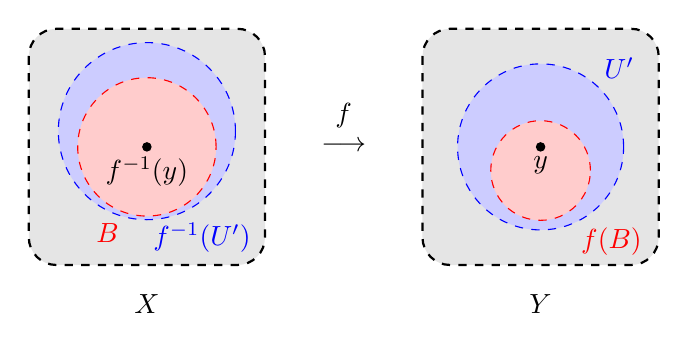
\begin{tikzpicture}
                    \def\incolor{gray!20}
        
                    \filldraw[rounded corners=10pt, dashed, thick, fill=\incolor] (0,0) rectangle (3,-3);
        
                    \node at (1.5, -3.5) {$X$};
                    \node at (4, -1.1) {$f$};
                    \node at (4, -1.5) {$\longrightarrow$};
        
                    \filldraw[rounded corners=10pt, dashed, thick, fill=\incolor] (5,0) rectangle (8,-3);
        
                    \node at (6.5, -3.5) {$Y$};
                    
                    \filldraw[dashed, draw=blue, fill=blue!20] (1.5, -1.3) circle (32pt);

                    \node at (2.2, -2.65) {\textcolor{blue}{$f^{-1}(U')$}};

                    \filldraw[dashed, draw=red, fill=red!20] (1.5, -1.5) circle (25pt);
        
                    \node at (1, -2.6) {\textcolor{red}{$B$}};
        
                    \filldraw[dashed, draw=blue, fill=blue!20] (6.5, -1.5) circle (30pt);
        
                    \filldraw[dashed, draw=red, fill=red!20] (6.5, -1.8) circle (18pt);
        
                    \node at (7.4, -2.7) {\textcolor{red}{$f(B)$}};
        
                    \node at (7.5, -0.5) {\textcolor{blue}{$U'$}};
        
                    \filldraw (1.5, -1.5) circle (1.5pt)  node[below] {$f^{-1}(y)$};
        
                    \filldraw (6.5, -1.5) circle (1.5pt)  node[below] {$y$};
        
                    
                \end{tikzpicture}
            \end{center}
            \item[(iv)] Sea $x\in X$, $N\in \cc{N}_x$. Como $\cc{N}_x$ es entorno, $\exists U\in \cc{T}$ con $x\in U\subset N' \Rightarrow f(x)\in f(U)\subset f(N)$ y como $f$ es abierta tengo que $f(U)\in \cc{T}'$ por lo que $f(N)\in \cc{N}_{f(x)}'$
            \item[(v)] Sea $N'\in \cc{N}_{f(x)}'$. Por (iv) (la implicación hacia la izquierda) tenemos que $f^{-1}(N')\in \cc{N}_x$. Como tenemos una b.d.e tenemos que $\exists V \in \cc{B}_x$ con $V\subset f^{-1}(N') \Rightarrow f(V)\subset N'$ y de nuevo por (iv) tenemos que $f(V)\in \cc{N}_{f(x)}'$ y tenemos lo que queríamos.
            \begin{center}
                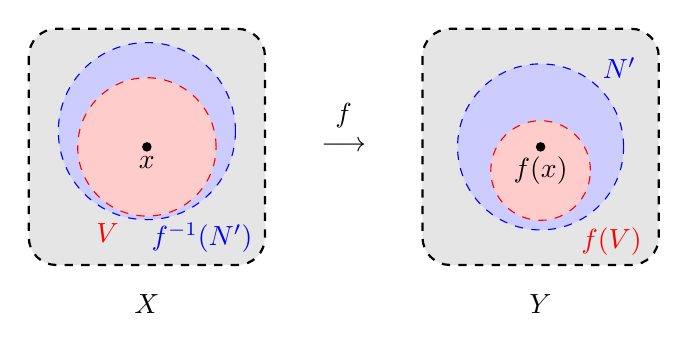
\begin{tikzpicture}
                    \def\incolor{gray!20}
        
                    \filldraw[rounded corners=10pt, dashed, thick, fill=\incolor] (0,0) rectangle (3,-3);
        
                    \node at (1.5, -3.5) {$X$};
                    \node at (4, -1.1) {$f$};
                    \node at (4, -1.5) {$\longrightarrow$};
        
                    \filldraw[rounded corners=10pt, dashed, thick, fill=\incolor] (5,0) rectangle (8,-3);
        
                    \node at (6.5, -3.5) {$Y$};
                    
                    \filldraw[dashed, draw=blue, fill=blue!20] (1.5, -1.3) circle (32pt);

                    \node at (2.2, -2.65) {\textcolor{blue}{$f^{-1}(N')$}};

                    \filldraw[dashed, draw=red, fill=red!20] (1.5, -1.5) circle (25pt);
        
                    \node at (1, -2.6) {\textcolor{red}{$V$}};
        
                    \filldraw[dashed, draw=blue, fill=blue!20] (6.5, -1.5) circle (30pt);
        
                    \filldraw[dashed, draw=red, fill=red!20] (6.5, -1.8) circle (18pt);
        
                    \node at (7.4, -2.7) {\textcolor{red}{$f(V)$}};
        
                    \node at (7.5, -0.5) {\textcolor{blue}{$N'$}};
        
                    \filldraw (1.5, -1.5) circle (1.5pt)  node[below] {$x$};
        
                    \filldraw (6.5, -1.5) circle (1.5pt)  node[below] {$f(x)$};
        
                    
                \end{tikzpicture}
            \end{center}
        \end{enumerate}
    \end{proof}
\end{prop}

\begin{definicion}
    Una propiedad $P$ que pueda o no tener un e.t. $(X, \cc{T})$ se dice \textbf{topológica} o que es un \textbf{invariante topológico} si al cumplirlo $(X, \cc{T})$, también la cumplen todos los espacios topológicos homeomorfos a él, es decir:
    \begin{gather*}
        (X, \cc{T}) \text{ cumple }P \sii (Y, \cc{T}') \text{ cumple } P\ \ \forall (Y, \cc{T}')\cong (X, \cc{T})
    \end{gather*}
    \endsquare
\end{definicion}

\begin{prop}
    Las propiedades \apuntar{T1}, \apuntar{T2}, \apuntar{1AN}, \apuntar{2AN} son invariantes topológicas.
    \begin{proof}
        Se deja como ejercicio para el lector %TODO: utilizar la proposición anterior (como la f es biyectiva son disjuntos)
    \end{proof}
\end{prop}

\begin{ejemplo}\
    \begin{itemize}
        \item $(\bb{R}, \cc{T}_u)\ncong (\bb{R}, \cc{T}_S)$ ya que $(\bb{R}, \cc{T}_u)$ es 2AN y $(\bb{R}, \cc{T}_S)$ no lo es.
        \item $(\bb{R}, \cc{T}_u)\ncong (\bb{R}, \cc{T}_{CF})\ncong (\bb{R}, \cc{T}_S)$ ya que $(\bb{R}, \cc{T}_u), (\bb{R}, \cc{T}_S)$ son T2 pero $(\bb{R}, \cc{T}_{CF})$ no lo es.
        \item $(\bb{R}, \cc{T}_u)\ncong (\bb{R}, \cc{T}_{disc})$ ya que $(\bb{R}, \cc{T}_{disc})$ no es 2AN.
    \end{itemize}
    \endsquare
\end{ejemplo}

\begin{definicion}
    Diremos que $f:(X, \cc{T})\to (Y, \cc{T}')$ es un \textbf{embebimiento} si $f^{f(X)}:(X, \cc{T})\to (f(X), \cc{T}_{f(X)}')$ es un homeomorfismo.
    En ese caso, $(X, \cc{T})\cong(f(X), \cc{T}_{f(X)}')$
    \endsquare
\end{definicion}

\begin{ejemplo}\
    \begin{itemize}
        \item $f$ homeomorfismo $\Rightarrow$ $f$ embebimiento. El recíproco no es cierto.
        \item Si $n, k \in \bb{N}$,
        \begin{align*}
            f:(\bb{R}^n, \cc{T}_u)&\to (\bb{R}^{n+k}, \cc{T}_u)\\
            x &\mapsto f(x)=(x,0)
        \end{align*}
        es un embebimiento con $f(\bb{R}^n)=\{\bb{R}^n \times \{0\}\}$.

        Para verlo tendremos que tomar la aplicación 
        \begin{align*}
            f^{\bb{R}^n\times \{0\}}:(\bb{R}^n, \cc{T}_u)&\to (\bb{R}^n\times \{0\}, \cc{T}_{u_{|\bb{R}^n\times \{0\}}})\\
            x &\mapsto (x,0)
        \end{align*}
        y tenemos además
        \begin{align*}
            (f^{\bb{R}^n\times \{0\}})^{-1}:(\bb{R}^n\times \{0\}, \cc{T}_{u_{|\bb{R}^n\times \{0\}}})&\to (\bb{R}^n, \cc{T}_u)\\
            (x,0) &\mapsto x
        \end{align*}
        y es fácil ver que $(f^{\bb{R}^n\times \{0\}})$ es un homeomorfismo y por tanto $f$ un embebimiento.
    \end{itemize}
    \endsquare
\end{ejemplo}

\section{Topología Producto}
En esta sección estudiaremos cómo a partir de dos e.t. $(X, \cc{T})$, $(Y, \cc{T}')$ podemos buscar una topología en el espacio $X\times Y$ a partir de $\cc{T}$ y $\cc{T}'$. Para ello, teniendo $X\times Y=\{(x,y):x\in X, y \in Y\}$ podemos tomar el conjunto $\{U\times U' : U\in \cc{T}, U'\in \cc{T}'\}$ pero vemos que no cumple la propiedad \apuntar{A2}. Sin embargo, sí podemos considerar que dicho conjunto sea una base de la topología producto.

\begin{prop}
    $\cc{B}_{\cc{T}\times \cc{T}'}=\{U\times U' : U\in \cc{T}, U'\in \cc{T}'\}$ es base de una única topología en $X\times Y$ que se denota $\cc{T}\times \cc{T}'$ y se llama \textbf{topología producto} de $\cc{T}$ y $\cc{T}'$. 

    Al e.t. $(X\times Y, \cc{T}\times \cc{T}')$ lo llamaremos \textbf{espacio topológico producto} de $(X, \cc{T})$ y $(Y, \cc{T}')$.

    \begin{proof} Para ver que esto es cierto tendremos que comprobar que cumple las condiciones de la Proposición %TODO 
        \begin{enumerate}
            \item[\apuntar{B1}] $X\times Y \in \cc{B}_{\cc{T}\times \cc{T}'}\Rightarrow \bigcup\limits_{B\in \cc{B}_{\cc{T}\times \cc{T}'}}=X\times Y$.
            \item[\apuntar{B2}] $U_1\times U_1', U_2\times U_2'\in \cc{B}_{\cc{T}\times \cc{T}'}$. Tenemos uqe $(U_1\times U_1')\cap (U_2\times U_2') = (U_1\cap U_2)\times (U_1'\times U_2')\in \cc{B}_{\cc{T}\times \cc{T}'}$. ya que $(U_1\times U_2)\in \cc{T}$ y $(U_1'\times U_2')\in \cc{T}'$.
        \end{enumerate}
        y ya lo tenemos probado.

    \end{proof}
\end{prop}

\begin{observacion}\
    \begin{itemize}
        \item Si $W\subset X\times Y$, $W\in \cc{T}\times \cc{T}'\sii \forall (x,y)\in W$\ \ $\exists U\in \cc{T}, U\in \cc{T}'$ con $(x,y)\in U\times U'\subset W \sii \forall (x,y)\in W\ \ \exists U\in \cc{T}, U'\in \cc{T}'$ con $x\in , y \in U', U\times U'\subset W \sii W=\bigcup\limits_{i\in I}U_i\times U_i'$ con $U_i\in \cc{T}, U_i'\in \cc{T}'\ \ \forall i\in I$.
        \item En $(X\times Y, \cc{T}\times \cc{T}')$, todo producto de abiertos es abierto (básico) pero el recíproco no es cierto ya que hay abiertos en el producto que no son procducto de abiertos. Es decir, que la topología $\cc{T}\times \cc{T}'$ hay más abiertos en general que los básicos, es decir, $\cc{T}\times \cc{T}'\setminus \cc{B}_{\cc{T}\times \cc{T}'}\neq \emptyset$.
    \end{itemize}
\end{observacion}

\begin{prop}
    Sean $(X, \cc{T}), (Y, \cc{T}')$ dos e.t. Entonces:
    \begin{enumerate}
        \item[(i)] Si $\cc{B}$ es base de $\cc{T}$ y $\cc{B}'$ es base de $\cc{T}'$, entonces $\tilde{\cc{B}}=\cc{B}\times \cc{B}'=\{B\times B': B\in \cc{B}, B'\in \cc{B}'\}$ es base de $\cc{T}\times \cc{T}'$.
        \item[(ii)] Si $x\in X$, $\cc{B}_x$ b.d.e. de $x$ en $(X, \cc{T})$ y $y\in Y$, $\cc{B}_y'$ b.d.e. de $y$ en $(Y, \cc{T}')$, entonces
        \begin{gather*}
            \tilde{\cc{B}}_{(x,y)}=\cc{B}_x\times \cc{B}_y' =\{V\times V': V\in \cc{B}_x, V'\in \cc{B}_y'\}
        \end{gather*}
        es b.d.e. de $(x,y)$ en $(X\times Y, \cc{T}\times \cc{T}')$.
    \end{enumerate}
    \begin{proof}\
        \begin{enumerate}
            \item[(i)] $\tilde{\cc{B}}=\cc{B}\times \cc{B}'\subset \cc{T}\times \cc{T}'$. Sea $W\in \cc{T}\times \cc{T}'$ y $(x,y)\in W$. Tendremos que ver que existe un elemento $B\times B'\in \tilde{\cc{B}}$ con $(x,y)\in B\times B'\subset W$. Como $\cc{B}_{\cc{T}\times \cc{T}'}$ es base de $\cc{T}\times \cc{T}'$, entonces $\exists U\in \cc{T}, U'\in \cc{T}'$ con $(x,y)\in U\times U'\subset W$. Como además $\cc{B}, \cc{B}'$ con bases tenemos que $\exists B\in \cc{B}, B'\in \cc{B}'$ con $x\in \cc{B}\subset U, y \in N'\subset U\Rightarrow (x,y)\in B\times B'\subset U\times U'\subset W$ y lo tenemos.
            \item[(ii)] La demostración es análoga a la anterior y se deja planteada como ejercicio para el lector.
        \end{enumerate}
    \end{proof}
\end{prop}

\begin{coro}
    $(X, \cc{T})$, $(Y, \cc{T})$ e.t.
    \begin{enumerate}
        \item[(i)] Si $(X, \cc{T})$ y $(Y, \cc{T}')$ son 1AN, entonces $(X\times Y, \cc{T}\times \cc{T}')$ es 1AN.
        \item[(ii)] Si $(X, \cc{T})$ y $(Y, \cc{T}')$ son 2AN, entonces $(X\times Y, \cc{T}\times \cc{T}')$ es 2AN.
    \end{enumerate}
    \endsquare
\end{coro}

\begin{ejemplo}\
    \begin{itemize}
        \item $\emptyset\neq A\subset X$, $\emptyset\neq A'\subset Y$ tenemos que $(\cc{T}, \cc{T}')_{|A\times A'}=\cc{T}_A \times \cc{T}_{A'}'$ (es fácil de comprobar).
        \item $\cc{T}_t\times \cc{T}_t = \cc{T}_t$.
        \item $\cc{T}_{disc}\times \cc{T}_{disc}=\cc{T}_{disc}$.
        \item $(\bb{R}^n\times \bb{R}^m, \cc{T}_u^n\times \cc{T}_u^m) = (\bb{R}^{n+m}, \cc{T}_u^{n+m})$.
        
        $B_{\infty}^n(x, \veps)\times B_{\infty}^m(y, \veps) = B_{\infty}^{n+m}((x,y), \veps)$.
    \end{itemize}
\end{ejemplo}
